\chapter*{Appendix: Comparison metrics of probabilistic data products \label{chap:append}}



We develop some intuition for the Kullback-Leibler Divergence by contrasting it with the familiar metric of the root-mean-square error (RMSE)
\begin{align}
\eqlabel{eq:rmse}
\mathrm{RMSE} &= \sqrt{\int (P(z) - \hat{P}(z))^{2} dz}.
\end{align}
Consider the simple example of a Gaussian $P(z) = \mathcal{N}(\mu_{0}, 
\sigma_{0}^{2})$ being approximated by a Gaussian $\hat{P}(z) = 
\mathcal{N}(\mu, \sigma^{2})$, whose KLD is
\begin{align}
\eqlabel{eq:gaussian}
\mathrm{KLD} &= \frac{1}{2}\left(\log\left[\frac{\sigma^{2}}{\sigma_{0}^{2}}\right] + \frac{\sigma_{0}^{2}}{\sigma^{2}} + \frac{(\mu - \mu_{0})^{2}}{\sigma^{2}} - 1\right)
\end{align}
To get a sense of the units of information, we can calculate the KLD and RMSE in some limiting cases.
If $\sigma = \sigma_{0}$ but $\mu = \mu_{0}+1$, we obtain $\mathrm{KLD} = \frac{1}{2}$ nat -- if the mean of the approximation is wrong by an additive factor of $\sigma$, half a nat of information is lost.
If $\mu = \mu_{0}$ but $\sigma = \sqrt{2\pi}\sigma_{0}$, we find $\mathrm{KLD} \approx \frac{1}{2}$ nat -- half a nat of information is also lost if the variance of the approximation is off by a multiplicative factor of $2\pi$.

We can use the KLD to identify notions of imprecision and inaccuracy.
Intuitively, precision must be related to how close $\sigma$ is to $\sigma_{0}$ and accuracy must be related to how close $\mu$ is to $\mu_{0}$.

\begin{figure}
	\begin{center}
		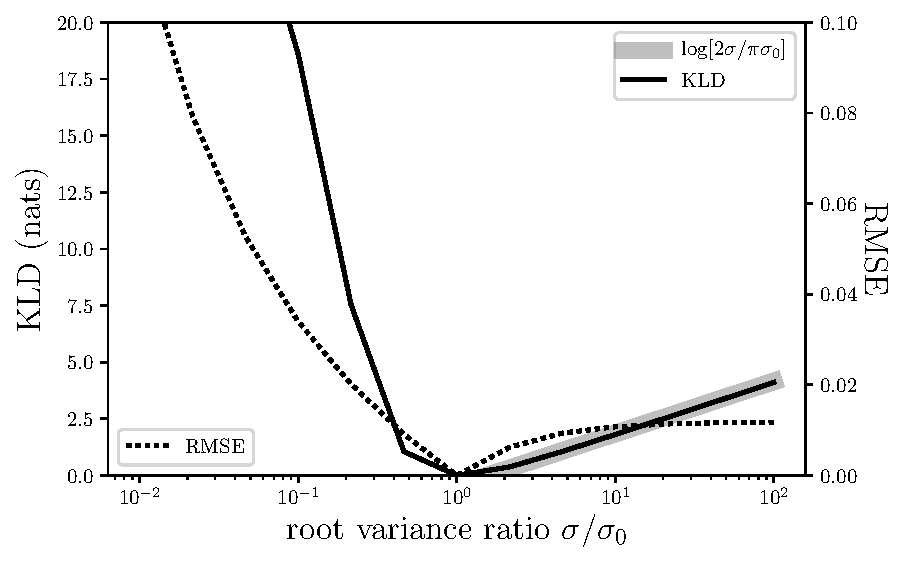
\includegraphics[width=0.74\columnwidth]{figures/qp/precision.pdf}
		\caption{The KLD and RMSE as a function of the root variance ratio $r$ for a simple Gaussian example.
			The KLD (solid line) rises sharply at $\sigma < \sigma_{0}$ and is proportional to the log of the inverse precision $r$ for $\sigma > \sigma_{0}$, behavior that is qualitatively similar to that of the RMSE (dotted line).
			\figlabel{fig:precision}}
	\end{center}
\end{figure}

If $\mu \approx \mu_{0}$, we can say $\mathrm{KLD}\sim\log[r] + \frac{1}{2}r^{-2} - \frac{1}{2}$ where $r^{-1} \equiv \frac{\sigma_{0}}{\sigma}$ is a measure of \textit{precision}, whose behavior is illustrated in \Fig{fig:precision}, alongside that of the RMSE.  
We observe that an overestimated variance increases the KLD as the log of the square root of the ratio of the estimated variance to the true variance.

\begin{figure}
	\begin{center}
		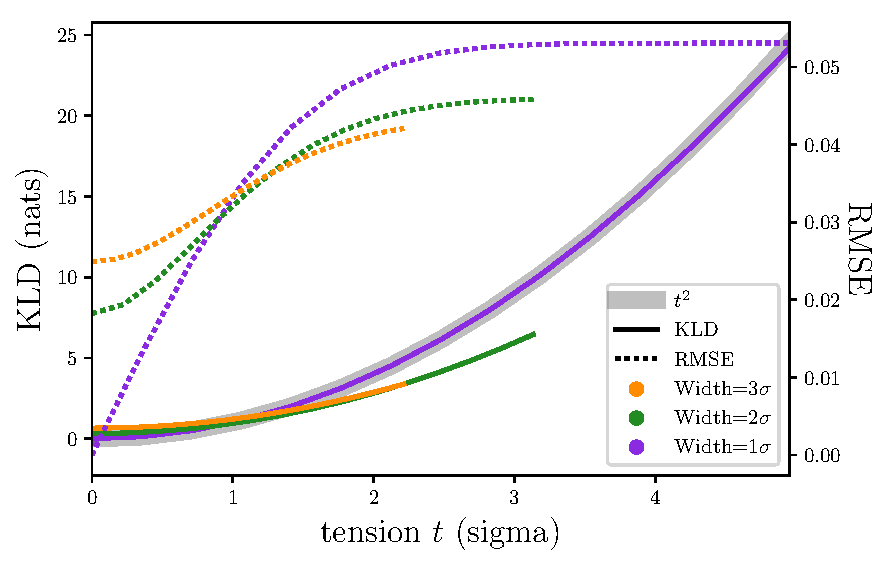
\includegraphics[width=0.74\columnwidth]{figures/qp/tension.pdf}
		\caption{The KLD and RMSE as a function of the tension $t$ for a simple Gaussian example.
			The KLD (solid lines) is equal to the square of the tension $t$, with a small offset when $r \neq 1$, whereas the RMSE (dotted lines) is relatively insensitive to tension past a certain point but more sensitive to $r \neq 1$.
			\figlabel{fig:tension}}
	\end{center}
\end{figure}

When $\sigma \approx \sigma_{0}$, $\mathrm{KLD} \sim t^{2}$ in terms of the \textit{tension} $t \equiv \frac{(\mu - \mu_{0})^{2}}{\sigma^{2}}$, whose concordance is illustrated in \Fig{fig:tension}.
There is some limiting tension $t_{\mathrm{lim}} \approx 2$ below which the RMSE is more sensitive than the KLD and above which the KLD is more sensitive than the RMSE.
This behavior hints at the KLD's reputation for sensitivity to the tails of the reference distribution.
The notion of tension may be more important for cosmological applications of \pz s, indicating the KLD may be a more appropriate metric for coarser approximations and the RMSE may be a more appropriate metric for less coarse approximations.
